This layer is the mount that control the release and hold of the tool.

\begin{figure}[h!]
	\centering
 	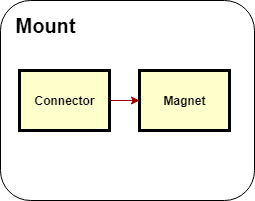
\includegraphics[width=0.60\textwidth]{images/Mount_Layer}
 \caption{Mount layer diagram}
\end{figure}

\subsection{Connector}
The connector is mounted on the wrist of the arm, but it is being control by the control box.

\subsubsection{Assumptions}
There is a 8 pin connector at the wrist of the arm and an available Lumberg RKMV 8-354 cable for the 8-pin connector.

\subsubsection{Responsibilities}
This connector control the mount to grab or release the tool by sending the magnet either 12v or 0v respectively.

\subsubsection{Subsystem Interfaces}
The connector interacts with the magnet by the instructions of the control box.

\begin {table}[H]
\caption {Connector interfaces} 
\begin{center}
    \begin{tabular}{ | p{1cm} | p{6cm} | p{3cm} | p{3cm} |}
    \hline
    ID & Description & Inputs & Outputs \\ \hline
    \#xx & Control Box & \pbox{3cm}{Voltage(0v or 12v)} & \pbox{3cm}{N/A}  \\ \hline
    \#xx & Magnet & \pbox{3cm}{N/A} & \pbox{3cm}{Voltage(0v or 12v}  \\ \hline
    \end{tabular}
\end{center}
\end{table}

\subsection{Magnet}
The magnet is place inside the mount where the tool can be inserted.

\subsubsection{Assumptions}
The magnet is strong enough to hold at least 5 pounds.
It receives either 0v or 12v from the UR5.
It does not takes more than 12v.

\subsubsection{Responsibilities}
The magnet is to grab/hold or release the tool by receiving either 0v or 12v.

\subsubsection{Subsystem Interfaces}
The magnet interface with the connector.

\begin {table}[H]
\caption {Magnet interfaces} 
\begin{center}
    \begin{tabular}{ | p{1cm} | p{6cm} | p{3cm} | p{3cm} |}
    \hline
    ID & Description & Inputs & Outputs \\ \hline
    \#xx & Connector & \pbox{3cm}{Voltage(0v or 12v)} & \pbox{3cm}{N/A}  \\ \hline
    \end{tabular}
\end{center}
\end{table}


